%=====================================================================
%  PROJET 1A — École des Ponts (CERMICS)
%  Réseaux de neurones pour la résolution d'EDP
%  PARTIE 1 (Paul Rivaud) : Introduction, état de l'art & méthode PINN
%
%  Thème : Beamer "Madrid" (identique au diaporama du groupe)
%  Compilation : pdflatex (2 passes) — ou latexmk -pdf
%=====================================================================
\documentclass[11pt,aspectratio=43]{beamer}

\usetheme{Madrid}                 % thème + couleur bleus identiques au template
\usepackage[utf8]{inputenc}
\usepackage[T1]{fontenc}
\IfFileExists{french.ldf}{\usepackage[french]{babel}}{} % typographie française (si le module est installé)
\usepackage{lmodern}              % polices Latin Modern (comme LaTeX par défaut)
\usepackage{amsmath,amssymb}
\usepackage{tikz}
\usetikzlibrary{positioning,arrows.meta,calc}

%---- POLICES : titres en sans-serif, corps de texte en serif (comme le template)
\setbeamerfont{normal text}{family=\rmfamily}
\setbeamerfont{frametitle}{family=\sffamily}
\setbeamerfont{title}{family=\sffamily}
\setbeamerfont{subtitle}{family=\sffamily}
\setbeamerfont{author}{family=\sffamily}
\setbeamerfont{date}{family=\sffamily}
\setbeamerfont{institute}{family=\sffamily}
\setbeamerfont{section in toc}{family=\sffamily}
\setbeamerfont{block title}{family=\sffamily}

%---- Couleurs exactes du template (bleu structure Beamer = RGB 51,51,178)
\definecolor{bblue}{RGB}{51,51,178}
\definecolor{dblue}{RGB}{38,38,134}

\setbeamertemplate{itemize items}[circle]   % puces rondes (comme le template)
\setbeamercovered{transparent}

%---- Métadonnées (les versions courtes [...] alimentent le bandeau du bas)
\title[PINNs et DeepRitz]{Résolution d'Équations Différentielles par Réseaux de Neurones}
\subtitle{Implémentation PyTorch des méthodes PINN et DeepRitz}
\author[Ait Abbou Soufiane, Paul Rivaud, Timoté Missaye, Pierre Kairo]{%
  Ait Abbou Soufiane, Paul Rivaud, Timoté Missaye, Pierre Kairo}
\date[6 juin 2026]{6 juin 2026}

%=====================================================================
\begin{document}

%--------------------------------------------------- 1. TITRE
\begin{frame}[plain]
  \titlepage
\end{frame}

%--------------------------------------------------- 2. PLAN
\begin{frame}{Plan de la présentation}
  \vfill
  \begin{enumerate}
    \setlength{\itemsep}{1.15em}
    \item Introduction \& méthode PINN \hfill {\small\itshape (cette partie)}
    \item Méthode Deep Ritz \& notre approche du problème
    \item Difficultés rencontrées \& présentation du code
    \item Résultats, optimisation des hyperparamètres \& conclusion
  \end{enumerate}
  \vfill
\end{frame}

%--------------------------------------------------- 3. CONTEXTE & MOTIVATION
\begin{frame}{Contexte \& motivation}
  \begin{itemize}
    \item Les \textbf{équations aux dérivées partielles (EDP)} modélisent
          d'innombrables phénomènes : mécanique, thermique, finance\ldots
    \item Mais très peu d'EDP admettent une \textbf{solution analytique} :
          on les résout \textbf{numériquement}.
  \end{itemize}
  \vfill
  \begin{block}{Problématique}
    \centering
    Peut-on résoudre une EDP en exploitant la puissance des
    \textbf{réseaux de neurones}, \emph{sans recourir à un maillage} ?
  \end{block}
\end{frame}

%--------------------------------------------------- 4. METHODES CLASSIQUES & LIMITES
\begin{frame}{Les méthodes classiques et leurs limites}
  \begin{columns}[T]
    \begin{column}{0.54\textwidth}
      \begin{itemize}
        \item Méthodes traditionnelles : \textbf{différences finies},
              \textbf{éléments finis}.
        \item Principe : \textbf{discrétiser} le domaine par un \textbf{maillage}.
        \item Limites :
          \begin{itemize}
            \item coût explosif en \textbf{grande dimension} ;
            \item géométries complexes, \textbf{remaillage}.
          \end{itemize}
      \end{itemize}
    \end{column}
    \begin{column}{0.46\textwidth}
      \centering
      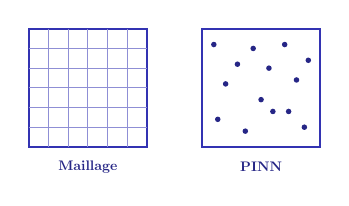
\begin{tikzpicture}[scale=0.50,font=\scriptsize,transform shape]
        \draw[bblue,thick] (0,0) rectangle (3,3);
        \foreach \i in {0.5,1,1.5,2,2.5}
          {\draw[bblue!55](\i,0)--(\i,3);\draw[bblue!55](0,\i)--(3,\i);}
        \node[text=dblue,font=\bfseries] at (1.5,-0.5){Maillage};
        \begin{scope}[xshift=4.4cm]
          \draw[bblue,thick] (0,0) rectangle (3,3);
          \foreach \p in {(0.4,0.7),(0.9,2.1),(1.5,1.2),(2.1,2.6),(2.6,0.5),
                          (1.1,0.4),(2.4,1.7),(0.6,1.6),(1.8,0.9),(2.7,2.2),
                          (1.3,2.5),(0.3,2.6),(2.2,0.9),(1.7,2.0)}
            {\fill[dblue]\p circle(2pt);}
          \node[text=dblue,font=\bfseries] at (1.5,-0.5){PINN};
        \end{scope}
      \end{tikzpicture}\\[1.2em]
      {\scriptsize\color{dblue} méthode classique \;vs\; sans maillage}
    \end{column}
  \end{columns}
  \vfill
  \begin{block}{Problème modèle — équation de Poisson 1D}
    \centering
    $\displaystyle -u''(x)=f(x)\ \text{ sur } ]0,1[\,,
      \qquad u(0)=u_0,\quad u(1)=u_1.$
  \end{block}
\end{frame}

%--------------------------------------------------- 5. POURQUOI DES RESEAUX
\begin{frame}{Pourquoi des réseaux de neurones ?}
  \begin{block}{1. Approximation universelle \textnormal{(Cybenko, 1989)}}
    Un réseau à \textbf{une seule couche cachée} et activation continue
    approxime \textbf{uniformément} toute fonction continue. On cherche donc
    la solution dans l'espace des réseaux :
    \[
      u_\theta(x)=\sum_{i=1}^{n} c_i\,\sigma(w_i\,x+b_i).
    \]
  \end{block}
  \begin{block}{2. Intégration de la physique \textnormal{(approche PINN)}}
    On incorpore l'EDP \emph{et} les conditions aux bords \textbf{directement}
    dans l'apprentissage. Cadre \textbf{non supervisé} : aucune donnée
    étiquetée, on minimise le \textbf{résidu} de l'EDP.
  \end{block}
\end{frame}

%--------------------------------------------------- 6. PRINCIPE DES PINN
\begin{frame}{Principe des PINN \textnormal{\small (Raissi, Perdikaris \& Karniadakis, 2019)}}
  \begin{itemize}
    \item Le réseau $u_\theta$ \emph{est} la solution approchée ; ses dérivées
          $u_\theta',\,u_\theta''$ sont obtenues par \textbf{différentiation automatique}.
    \item On transforme l'EDP en un \textbf{problème d'optimisation}.
  \end{itemize}
  \vfill
  \centering
  \resizebox{0.96\textwidth}{!}{%
  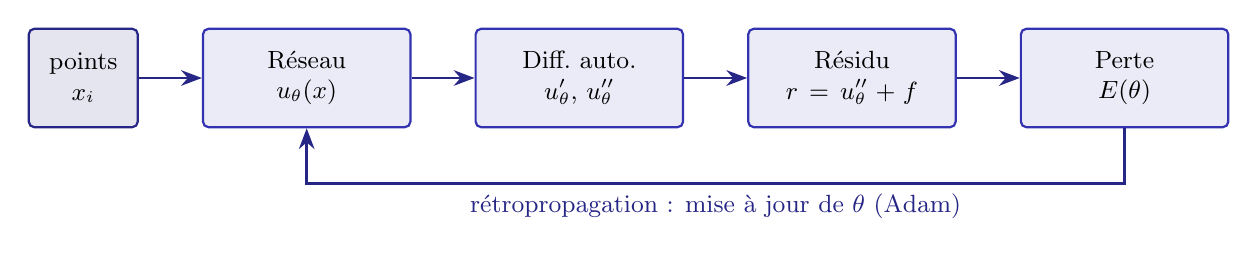
\begin{tikzpicture}[>=Stealth,node distance=0.6cm and 0.8cm,
    box/.style={rectangle,rounded corners=2pt,draw=bblue,fill=bblue!10,thick,
                minimum height=1.25cm,text width=2.4cm,align=center,font=\small},
    io/.style={rectangle,rounded corners=2pt,draw=dblue,fill=dblue!12,thick,
                minimum height=1.25cm,text width=1.15cm,align=center,font=\small},
    ar/.style={->,line width=1pt,draw=dblue}]
    \node[io] (x) {points $x_i$};
    \node[box,right=of x]   (net) {Réseau\\ $u_\theta(x)$};
    \node[box,right=of net] (ad)  {Diff.\ auto.\\ $u_\theta',\,u_\theta''$};
    \node[box,right=of ad]  (res) {Résidu\\ $r=u_\theta''+f$};
    \node[box,right=of res] (loss){Perte\\ $E(\theta)$};
    \draw[ar](x)--(net);\draw[ar](net)--(ad);\draw[ar](ad)--(res);\draw[ar](res)--(loss);
    \draw[ar] (loss.south) -- ++(0,-0.7) -|
      node[pos=0.25,below,font=\small,text=dblue]
      {rétropropagation : mise à jour de $\theta$ (Adam)} (net.south);
  \end{tikzpicture}}
\end{frame}

%--------------------------------------------------- 7. ARCHITECTURE DU RESEAU
\begin{frame}{Architecture du réseau}
  \begin{columns}[c]
    \begin{column}{0.50\textwidth}
      \centering
      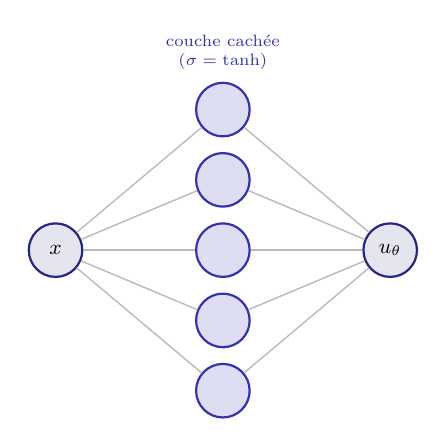
\begin{tikzpicture}[>=Stealth,scale=0.85,transform shape,font=\small,
        inp/.style={circle,draw=dblue,fill=dblue!12,minimum size=0.8cm,thick},
        hid/.style={circle,draw=bblue,fill=bblue!16,minimum size=0.8cm,thick},
        onode/.style={circle,draw=dblue,fill=dblue!12,minimum size=0.8cm,thick},
        edg/.style={draw=gray!55,line width=0.5pt}]
        \node[inp](x) at (0,0){$x$};
        \foreach \i/\y in {1/2.1,2/1.05,3/0,4/-1.05,5/-2.1}
          {\node[hid](h\i) at (2.5,\y){};}
        \node[onode](u) at (5,0){$u_\theta$};
        \foreach \i in {1,...,5}{\draw[edg](x)--(h\i);\draw[edg](h\i)--(u);}
        \node[text=bblue,align=center,font=\scriptsize] at (2.5,2.95)
              {couche cachée\\ ($\sigma=\tanh$)};
      \end{tikzpicture}
    \end{column}
    \begin{column}{0.50\textwidth}
      \begin{itemize}
        \item Espace des réseaux ($\theta\in\mathbb{R}^{3n}$) :
          \[ \textstyle V_{nn}=\bigl\{\,x\mapsto\sum_{i=1}^{n} c_i\,\sigma(w_ix+b_i)\bigr\} \]
        \item Activation $\sigma=\tanh$, donc $\sigma'(x)=1-\tanh^2(x)$.
        \item $C^\infty \Rightarrow u_\theta\in C^2$ et $u_\theta''$
              \textbf{calculable} par autodiff.
      \end{itemize}
    \end{column}
  \end{columns}
\end{frame}

%--------------------------------------------------- 8. FONCTION DE PERTE PHYSIQUE
\begin{frame}{La fonction de perte physique}
  La fonctionnelle d'énergie mesure à quel point $u_\theta$ viole l'EDP et les bords :
  \[
    E(u_\theta)=\int_{\Omega}\bigl|u_\theta''(x)+f(x)\bigr|^2dx
      +\bigl(u_\theta(0)-u_0\bigr)^2+\bigl(u_\theta(1)-u_1\bigr)^2 .
  \]
  En pratique (collocation sur $N$ points $x_i$) :
  \[
    \mathcal{L}(\theta)=
    \underbrace{\frac{1}{N}\sum_{i=1}^{N}\bigl(u_\theta''(x_i)+f(x_i)\bigr)^2}
      _{\textcolor{bblue}{\mathcal{L}_{\mathrm{PDE}}\ :\ \text{résidu de l'EDP}}}
    +\underbrace{\bigl(u_\theta(0)-u_0\bigr)^2+\bigl(u_\theta(1)-u_1\bigr)^2}
      _{\textcolor{bblue}{\mathcal{L}_{\mathrm{BC}}\ :\ \text{conditions aux bords}}}
  \]
  \begin{itemize}
    \item $u^\star$ solution exacte $\iff E(u^\star)=0$, d'où
          $\displaystyle \theta^\star=\arg\min_{\theta}\mathcal{L}(\theta)$.
    \item Minimisation par \textbf{descente de gradient (Adam)} ;
          $\nabla_\theta\mathcal{L}$ obtenu par \textbf{rétropropagation}.
  \end{itemize}
\end{frame}

%--------------------------------------------------- 9. CONCLUSION DE PARTIE
\begin{frame}{Conclusion de partie \& transition}
  \begin{itemize}
    \item Les PINN reformulent une EDP en un \textbf{problème d'optimisation} :
          le réseau apprend à \textbf{annuler le résidu} de l'équation.
    \item Atouts : \textbf{sans maillage}, \textbf{non supervisé}, adaptés
          aux grandes dimensions et aux problèmes inverses.
  \end{itemize}
  \vfill
  \begin{block}{Transition}
    \centering
    Place à la \textbf{méthode Deep Ritz} (formulation variationnelle)
    et à notre \textbf{implémentation PyTorch}.
  \end{block}
\end{frame}

\end{document}
